\documentclass[notitlepage]{article}

\usepackage{bibunits}
\usepackage{comment}
\usepackage{graphicx}
\usepackage{amsmath}
\usepackage{bm}
\usepackage{amssymb}
\usepackage{datetime}
\usepackage{numprint}

% processes above options
\usepackage{palatino}  %OR newcent ncntrsbk helvet times palatino
\usepackage{url}
\usepackage{footmisc}
\usepackage{endnotes}
\usepackage{graphicx}
\graphicspath{{/home/esteban/Desktop/school/fall2023/compVar/hw2}}

\newcommand{\HwBreak}{%
  \par\noindent\makebox[\linewidth]{\rule{0.9\paperwidth}{0.4pt}}\par%
}


\setcounter{secnumdepth}{3}
\begin{document}

\nplpadding{2}
\newdateformat{isodate}{
  \THEYEAR -\numprint{\THEMONTH}-\numprint{\THEDAY}}
  
\title{Homework 2}
\author{Esteban Calvo}
\date{\isodate\today}

\maketitle

\newpage
\section*{Exercise 1}
    To prove that $f(z)=e^{\bar{z}}$ is not differentiable anywhere, we can show that the partial derivates for Cauchy-Reimann to hold are not equal. 
    We can start by expanding out the function as follows
   \begin{equation}
    \begin{aligned}
        e^{\bar{z}} &= e^x*e^{-iy} \notag \\
                    &= e^x(cos(y)+isin(-y) \\
                    &= e^x(cos(y)-isin(y)) \\
                    &= e^xcos(y) - e^xisin(y)
    \end{aligned}
\end{equation}
    From here, we can get the following equaitons
\begin{equation}
    \begin{aligned}
                u   &= e^xcos(y) \notag\\
                v   &= -e^xsin(y)
    \end{aligned}
\end{equation}
    We can then use u and v for the partial derivatives as follows
\begin{equation}
    \begin{aligned}
        \frac{\partial u}{\partial x} &= e^xcos(y)\notag \\
        \frac{\partial v}{\partial y} &= -e^xsin(y)
    \end{aligned}
\end{equation}
    Thus, we see that the partial derivatives are not equal and thus the function is not analytical anywhere \\~\\

\HwBreak

\section*{Exercise 2}
    The definition for the principal log is as follows
    $$Log(z) = ln(|z|) + iarg(z)$$
    Thus, we can use both $i^3$ and $i$ to see if the results differ. First, we can start with $Log(i^3)$ as follows.
   \begin{equation}
    \begin{aligned}
        Log(i^3)    &= ln(|i^3|) + i arg(i^3) \notag \\
                    &= ln(i) -\frac{3i\pi}{2}
    \end{aligned}
\end{equation}
    We can now try with $3Log(i)$ as follows
 \begin{equation}
    \begin{aligned}
        3Log(i)    &= 3(ln(|i|) + i arg(i)) \notag \\
                    &= 3ln(i) + \frac{3i\pi}{2}
    \end{aligned}
\end{equation}
    Therefore, we can see that $$3ln(i) + \frac{3i\pi}{2} \neq ln(i) -\frac{3i\pi}{2}$$ and therefore we cannot factor out the exponent as with regular log functions for non-complex functions. \\~\\

    \HwBreak
\section*{Exercise 3}
    \subsection*{a)}
    To begin, we want to prove $sin(z) = sin(x+iy) = sin(x)cosh(y)+icos(x)sinh(y)$ and to do this we can use the following identities
    \begin{equation}
        \begin{aligned}
            & sin(z)= \frac{1}{2i}(e^{iz}-e^{-iz})\\
            & sinh(y) = \frac{1}{2}(e^y-e^{-y}) \\
            & cosh(y) = \frac{1}{2}(e^y+e^{y}) \\
            & e^{ix} = cos(x) + isin(x)
        \end{aligned}
    \end{equation} \\
    We can expand out sin(z) using (1) and then expand out z as $z=x+iy$ to get the following equation 
    $$\frac{1}{2i}(e^{i(x+iy)}-e^{-i(x+iy)}$$
    From here, we can begin to factor and combine like terms as follows
    \begin{equation}
        \begin{aligned}
            & \frac{1}{2i}(e^{ix}e^{-y}-e^{-ix}e^y)\notag \\
            & \frac{1}{2i}([cos(x)+isin(x)]e^{-y}-[cos(x)-isin(x)]e^y) \\
            & (\frac{e^{-y}-e^y}{2i})cos(x)+isin(x)(\frac{e^y+e^{-y}}{2}) \\
            & sin(x)cosh(y)+icos(x)sinh(y)
        \end{aligned}
    \end{equation}
    \subsection*{b)}
    We now want to prove that $|sin(z)|^2 = sin^2(x)+sinh^2(y)$. To begin, we can expand out sin(z) using the previously found identity
   \begin{equation}
    \begin{aligned}
       |sin(z)|^2  &= |sin(x)cosh(y) + icos(x)sinh(y)|^2\notag \\
                   &= |sin(x)cosh(y)|^2+|cos(x)sinh(y)|^2 \\
                   &= sin^2(x)cosh(y)^2 + cos^2(x)sinh^2(y)\\
                   &= sin^2(x)cosh^2(y) + cos^2(x)(cosh^2(y)-1)\\
                   &= cosh^2(y) - (1-sin^2(x))\\
                   &= (sinh^2(y)+1) - (1-sin^2(y))\\
                   &= sin^2(x) + sinh^2(y)
    \end{aligned}
\end{equation}
    \subsection*{c)}
    If we want to find the zeroes of the complex function sin(z) which is in the form of $ sin(z)= \frac{1}{2i}(e^{iz}-e^{-iz}$, we want to show that $sin(z) = 0$.
    This is only possible when $e^{iz}-e^{-iz}=0$ and thus we need to see where $e^{iz}=e^{-iz}$ and thus $e^{2iz}=1$ For this to be the case, we must have the following 
    constraints $z=n \pi , n \in \mathbb{Z}$ \\~\\

\HwBreak
\section*{Exercise 4}
    \subsection*{a)}
    To find that $sin(\bar{z})$ is not analytic anywhere, we can use the identity found in exercise 3 as follows
\begin{equation}
    \begin{aligned}
        sin(\bar{z})    &= sin(x)cosh(y)-icos(x)sinh(y) \notag \\
        u               &= sin(x)cosh(y) \\
        v               &= -cos(x)sinh(y)
    \end{aligned}
\end{equation}
    We can then use Cauchy-Reimann as follows
\begin{equation}
    \begin{aligned}
        \frac{\partial u}{\partial x} &= cos(x)cosh(y) \notag \\
        \frac{\partial v}{\partial y} &= -cos(x)cosh(y)
    \end{aligned}
\end{equation}
    We can therefore see that the two partial derivates are not equal and therefore Cauchy-Reimann does not hold
    \subsection*{b)}
    A similar identity for cos(z) exists $cos(z) = cos(x)cosh(y)-isin(x)sinh(y)$ which we can use to find the conjugate and take partial derivates for
    \begin{equation}
    \begin{aligned}
        cos(\bar{z})    &=  cos(x)cosh(y) + isin(x)sinh(y) \notag \\
        u               &= cos(x)cosh(y) \\
        v               &= sin(x)sinh(y)
    \end{aligned}
\end{equation}
    Taking the partials yields the following results
\begin{equation}
    \begin{aligned}
        \frac{\partial u}{\partial x} &= -sin(x)cosh(y) \notag \\
        \frac{\partial v}{\partial y} &= sin(x)cosh(y)
    \end{aligned}
\end{equation}
    And thus the partials are once again not equal therefore $cos(\bar{z})$ is not analytical anywhere \\~\\
    
\HwBreak
\section*{Exercise 5}
    We are told to use the following definitions \\
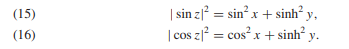
\includegraphics[width=4in]{ex5_1} \\
    to show that $|sin(z)| \geq |sin(x)|$ and $|cos(z)| \geq |cos(x)|$
    \subsection*{a)}
    We can use (15) to show that $|sin(z)|^2$ must be greater than or equal to $|sin(x)|^2$ by using modulus properties.
    Using modulus properties, we can rewrite both funtions as follows
\begin{equation}
    \begin{aligned}
        |sin(z)|^2  &= Re(sin(z))^2+Im(sin(z))^2 \notag \\
        |sin(x)|^2  &= Re(sin(x))^2 + Im(sin(x))^2
    \end{aligned}
\end{equation}
    Using identity 15 and the fact that there is no imaginary part of sin(x), we can rewrite as follows
\begin{equation}
    \begin{aligned}
        |sin(z)|^2  &= sin^2(x) + sinh^2(y) \notag \\
        |sin(x)|^2  &= sin^2(x)
    \end{aligned}
\end{equation}
    Because we know that $sinh^2(y) \geq 0$, we can therefore state that $|sin(z)|^2 \geq |sin(x)|^2$ and therefore $|sin(z)| \geq |sin(x)|$

    \subsection*{b)}
    We can now begin to prove $|cos(z)| \geq |cos(x)|$ using similar logic as follows.
\begin{equation}
    \begin{aligned}
        |cos(z)|^2  &= cos^2(x)+sinh^2(y) \notag \\
        |cos(x)|^2  &= cos^2(x)
    \end{aligned}
\end{equation}
    We can apply the same logic as before that $cosh^2(y) \geq 0$ because the function is squared and therefore it follows that
    $|cos(z)|^2 \geq |cos(x)|^2$ thus $|cos(z)| \geq |cos(x)|$ \\~\\

\HwBreak
\section*{Exercise 6}
    \subsection*{a)} 
    Given: $|sinh(y)| \leq |sin(z)| \leq |cosh(y)|$
    Proof: \\
    We are given that $|sin(z)|^2 = sin^2(x) + sinh^2(y)$ and similar to the last proof we can see that because $|sin(z)|^2$ includes $sinh^2(y)$, it must be greather than
    or equal to $sinh^2(y)$ because $sin^2(x)$ is positive everywhere. We now must use the modulus definition as follows
\begin{equation}
    \begin{aligned}
        |sin(z)|^2  &= sin^2(x) + sinh^2(y) \notag \\
                    &= sin^2(x) + cosh^2(y)-1 \\
                    &= cosh^2(y) - (1 - sin^2(x)) \\
                    &= cosh^2(y) - cos^2(x)
    \end{aligned}
\end{equation}
    We know that $cos^2(x) \geq 0$ and therefore we know that $cosh^2(y)$ must be greater than $|sin(z)|^2$ for this inequality to hold. Therefore, we can combine all three parts to get
    $$|sinh(y)| \leq |sin(z)|^2 \leq cosh(y)$$
     
     \subsection*{b)}
     Given: $|sinh(y)| \leq |cos(z)| \leq |cosh(y)|$
    Proof: \\
    We are given that $|cos(z)|^2 = cos^2(x) + sinh^2(y)$ and therefore we can once again see that $|cos(z)|$ will be larger as $|cos(z)|^2 \geq sinh^2(y)$. We can also show that 
    $cosh(y)$ as follows
\begin{equation}
    \begin{aligned}
        |cos(z)|^2  &= cos^2(x) + sinh^2(y) \notag \\
                    &= cos^2(x) + cosh^2(y)-1 \\
                    &= cosh^2(y) - (1 - cos^2(x)) \\
                    &= cosh^2(y) - sin^2(x)
    \end{aligned}
\end{equation}
    We once again see that for this inequality to hold, $cosh^2(y)$ must be larger since $sin^2(x) \geq 0$. Therefore, we get 
    $$|sinh(y)| \leq |cos(z)| \leq |cosh(y)|$$ \\
    
\HwBreak
\section*{Exercise 7}
\subsection*{a)}
    Identity: $-isinh(iz)=sin(z)$ \\
    Proof: \\
\begin{equation}
    \begin{aligned}
        -isinh(z)   &= \frac{-i}{2}(e^{iz}-e^{-iz}) \notag \\
                    &= \frac{-i}{2}([cos(z)+isin(z)] - [cos(z)-isin(z)])\\
                    &= \frac{-i}{2}(2isin(z))\\
                    &= sin(z)
    \end{aligned}
\end{equation}
\subsection*{b)}
    Identity: $-isin(iz)=sinh(z)$ \\
    Proof: \\
\begin{equation}
    \begin{aligned}
        -isin(iz)   &= \frac{i}{2i}(e^{i^2z}-e^{-i^2z})\ \notag \\
                    &= \frac{-1}{2}(e^{-z}-e^z)\\
                    &= \frac{1}{2}(e^z-e^{-z})\\
                    &= sinh(z)
    \end{aligned}
\end{equation}

\subsection*{c)}
    Identity: $cos(iz) = cosh(z)$ \\
    Proof: \\
\begin{equation}
    \begin{aligned}
        cos(iz)     &= \frac{1}{2}(e^{i^2z}+e^{-i^2z}) \notag \\
                    &= \frac{1}{2}(e^z+e^{-z}) 
                    &= cosh(z)
    \end{aligned}
\end{equation} 

\section*{Exercise 8}
\subsection*{a)}
    Identity: $sinh(z) = sinh(x)cos(y) + icosh(x)sin(y)$ \\
    Proof: \\
\begin{equation}
    \begin{aligned}
        sinh(z)     &= \frac{1}{2}(e^z-e^{-z}) \notag \\
                    &= \frac{1}{2}(e^xe^{iy}-e^{-x}e^{-iy}) \\
                    &= \frac{1}{2}(e^x(cos(y)+isin(y)) - e^{-x}(cos(y)-isin(y))) \\
                    &= \frac{1}{2}((e^x-e^{-x})cos(y)+(e^x+e^{-x})isin(y)) \\
                    &= \frac{(e^x-e^{-x})cos(y)}{2} + \frac{(e^x+e^{-x})isin(y)}{2} \\
                    &= sinh(x)cos(y) + icosh(x)sin(y)
    \end{aligned}
\end{equation}

\subsection*{b)}
    Identity: $cosh(z) = cosh(x)cos(y) + isinh(x)sin(y)$ \\
    Proof: \\
\begin{equation}
    \begin{aligned}
        cosh(z)     &= \frac{1}{2}(e^z+e^{-z})\notag \\
                    &= \frac{1}{2}(e^xe^{iy}+e^{-x}e^{-iy}) \\
                    &= \frac{1}{2}(e^x(cos(y)+isin(y)) + e^{-x}(cos(y)-isin(y))) \\
                    &= \frac{1}{2}((e^x+e^{-x})cos(y)+(e^x-e^{-x})isin(y)) \\
                    &= \frac{(e^x+e^{-x})cos(y)}{2} + \frac{(e^x-e^{-x})isin(y)}{2} \\
                    &= cosh(x)cos(y) + isinh(x)sin(y) 
    \end{aligned}
\end{equation}

\subsection*{c)}
    Identity: $|sinh(z)|^2 = sinh^2(x) + sin^2(x)$ \\
    Useful Identity: $|z|^2 = Re(z)^2 + Im(z)^2$
    Proof: \\
\begin{equation}
    \begin{aligned}
        |sinh(z)|^2     &= (sinh(x)cos(y))^2+(cosh(x)sin(y))^2 \notag \\
                        &= sinh^2(x)cos^2(y) + cosh^2(x)sin^2(y) \\
                        &= (cosh^2(x)-1)cos^2(y) + sin^2(y)cosh^2(x) \\
                        &= cosh^2(x)(cos^2(y)+sin^2(x)) - cos^2(y) \\
                        &= cosh^2(x) - cos^2(y) \\
                        &= sinh^2(x) + (1 - cos^2(y)) \\
                        &= sinh^2(x) + sin^2(y)
    \end{aligned}
\end{equation}

\subsection*{d)}
    Identity: $|cosh(z)|^2 = sinh^2(x) + cos^2(y)$ \\
    Proof: \\
\begin{equation}
    \begin{aligned}
        |cosh(z)|^2     &= (cosh(x)cos(y))^2+(sinh(x)sin(y))^2 \notag \\
                        &= coshh^2(x)cos^2(y) + sinh^2(x)sin^2(y) \\
                        &= (sinh^2(x)+1)cos^2(y) + sin^2(y)sinh^2(x) \\
                        &= sinh^2(x)(sin^2(y)+sin^2(y)) + cos^2(y) \\
                        &= sinh^2(x) + cos^2(y)
    \end{aligned}
\end{equation} \\~\\

\HwBreak
\section*{Exercise 9}
 To take the integral of a complex function, we must use the following form
    $$\int_a^b{u(t)+iv(t)dt} = \int_a^b{u(t)dt} + i \int_a^b{v(t)dt}$$

\subsection*{a)}
    Problem: $\int_0^1{(1+it)^2dt}$
    Solution: \\
\begin{equation}
    \begin{aligned}
        \int_0^1{(1+it)^2dt}    &= \int_0^1{1+2it-t^2dt} \notag \\
                                &= \int_0^1{1-t^2dt} + i\int_0^1{2tdt} \\
                                &= \left[t-\frac{t^3}{3}\right]_0^1 + i\left[\frac{2t^2}{2}\right]_0^1 \\
                                &= \frac{2}{3} + i
    \end{aligned}
\end{equation}

\subsection*{b)}
    Problem: $\int_1^2{(\frac{1}{t}-i)^2dt}$
    Solution: \\
\begin{equation}
    \begin{aligned}
        \int_1^2{(\frac{1}{t}-i)^2dt}   &= \int_1^2{\frac{1}{t^2}-1-\frac{2}{t}} \notag \\
                                        &= \int_1^2{\frac{1}{t^2}-1dt} + i\int_1^2{-\frac{2}{t}dt} \\
                                        &= \left[-(\frac{1}{t}+t)\right]_1^2 - i\left[ln(t^2)\right]_1^2 \\
                                        &= -\frac{1}{2} - iln(4)
    \end{aligned}
\end{equation}

\subsection*{c)}
    Problem: $\int_0^\pi{e^{i2t}dt}$
    Solution: \\
\begin{equation}
    \begin{aligned}
       \int_0^\pi{e^{i2t}dt}    &= \int_0^\pi{cos(2t)+isin(2t)dt} \notag \\
                                &= \int_0^\pi{cos(2t)dt} + i\int_0^\pi{sin(2t)dt} \\
                                &= \left[\frac{sin(2t)}{2}\right]_0^{\pi/6} - i\left[\frac{cos(2t)}{2}\right]_0^{\pi/6} \\
                                &= \frac{\sqrt 3}{4} + \frac{i}{4}
    \end{aligned}
\end{equation}

\subsection*{d)}
    Problem: $\int_0^\infty{e^{-zt}dt}$
    Solution: \\
\begin{equation}
    \begin{aligned}
       \int_0^\infty{e^{-zt}dt}     &= \left[-\frac{e^{-zt}}{z}\right]_0^{\infty} \notag \\
                                    &= \frac{-e^{-\infty}}{z} + \frac{e^0}{z} \\
                                    &=\frac{1}{z}
    \end{aligned}
\end{equation} \\~\\


\HwBreak
\section*{Exercise 10}
    To prove the given conjecture, we need to examine the integral when $m=n$ and when $m \neq n$
\subsection*{m=n}
\begin{equation}
    \begin{aligned}
        \int_0^{2\pi}{e^{im\theta}e^{-im\theta}d\theta}     &=  \int_0^{2\pi}{e^{im\theta - im\theta}d\theta} \notag \\
                                                            &=  \int_0^{2\pi}{e^0d\theta} \\
                                                            &= \int_0^{2\pi}{1d\theta} \\
                                                            &= \left[\theta\right]_0^{2\pi} \\
                                                            &= 2\pi
    \end{aligned}
\end{equation} 

\subsection*{m not equal n}
\begin{equation}
    \begin{aligned}
        \int_0^{2\pi}{e^{im\theta}e^{-in\theta}d\theta}     &= \int_0^{2\pi}{e^{im\theta - in\theta}d\theta} \notag \\
                                                            &= \int_0^{2\pi}{e^{i(m-n)\theta}d\theta} \\
                                                            &= \left[\frac{e^{i(m-n)\theta}}{i(m-n)}\right]_0^{2\pi} \\
                                                            &= \frac{1}{1(m-n)}\left[cos((m-n)\theta)+isin((m-n)\theta)\right]_0^{2\pi} \\
                                                            &= \frac{1}{1(m-n)}(cos((m-n)2\pi)+isin((m-n)2\pi)-cos(0)-isin(0)) \\
                                                            &= \frac{1}{1(m-n)}(1+0-1-0) \\
                                                            &= 0
    \end{aligned}
\end{equation}
    Thus we have shown the conjecture to hold

\end{document}

